\title{DIY tinyUSBboard}
\subtitle{Lötanleitung}
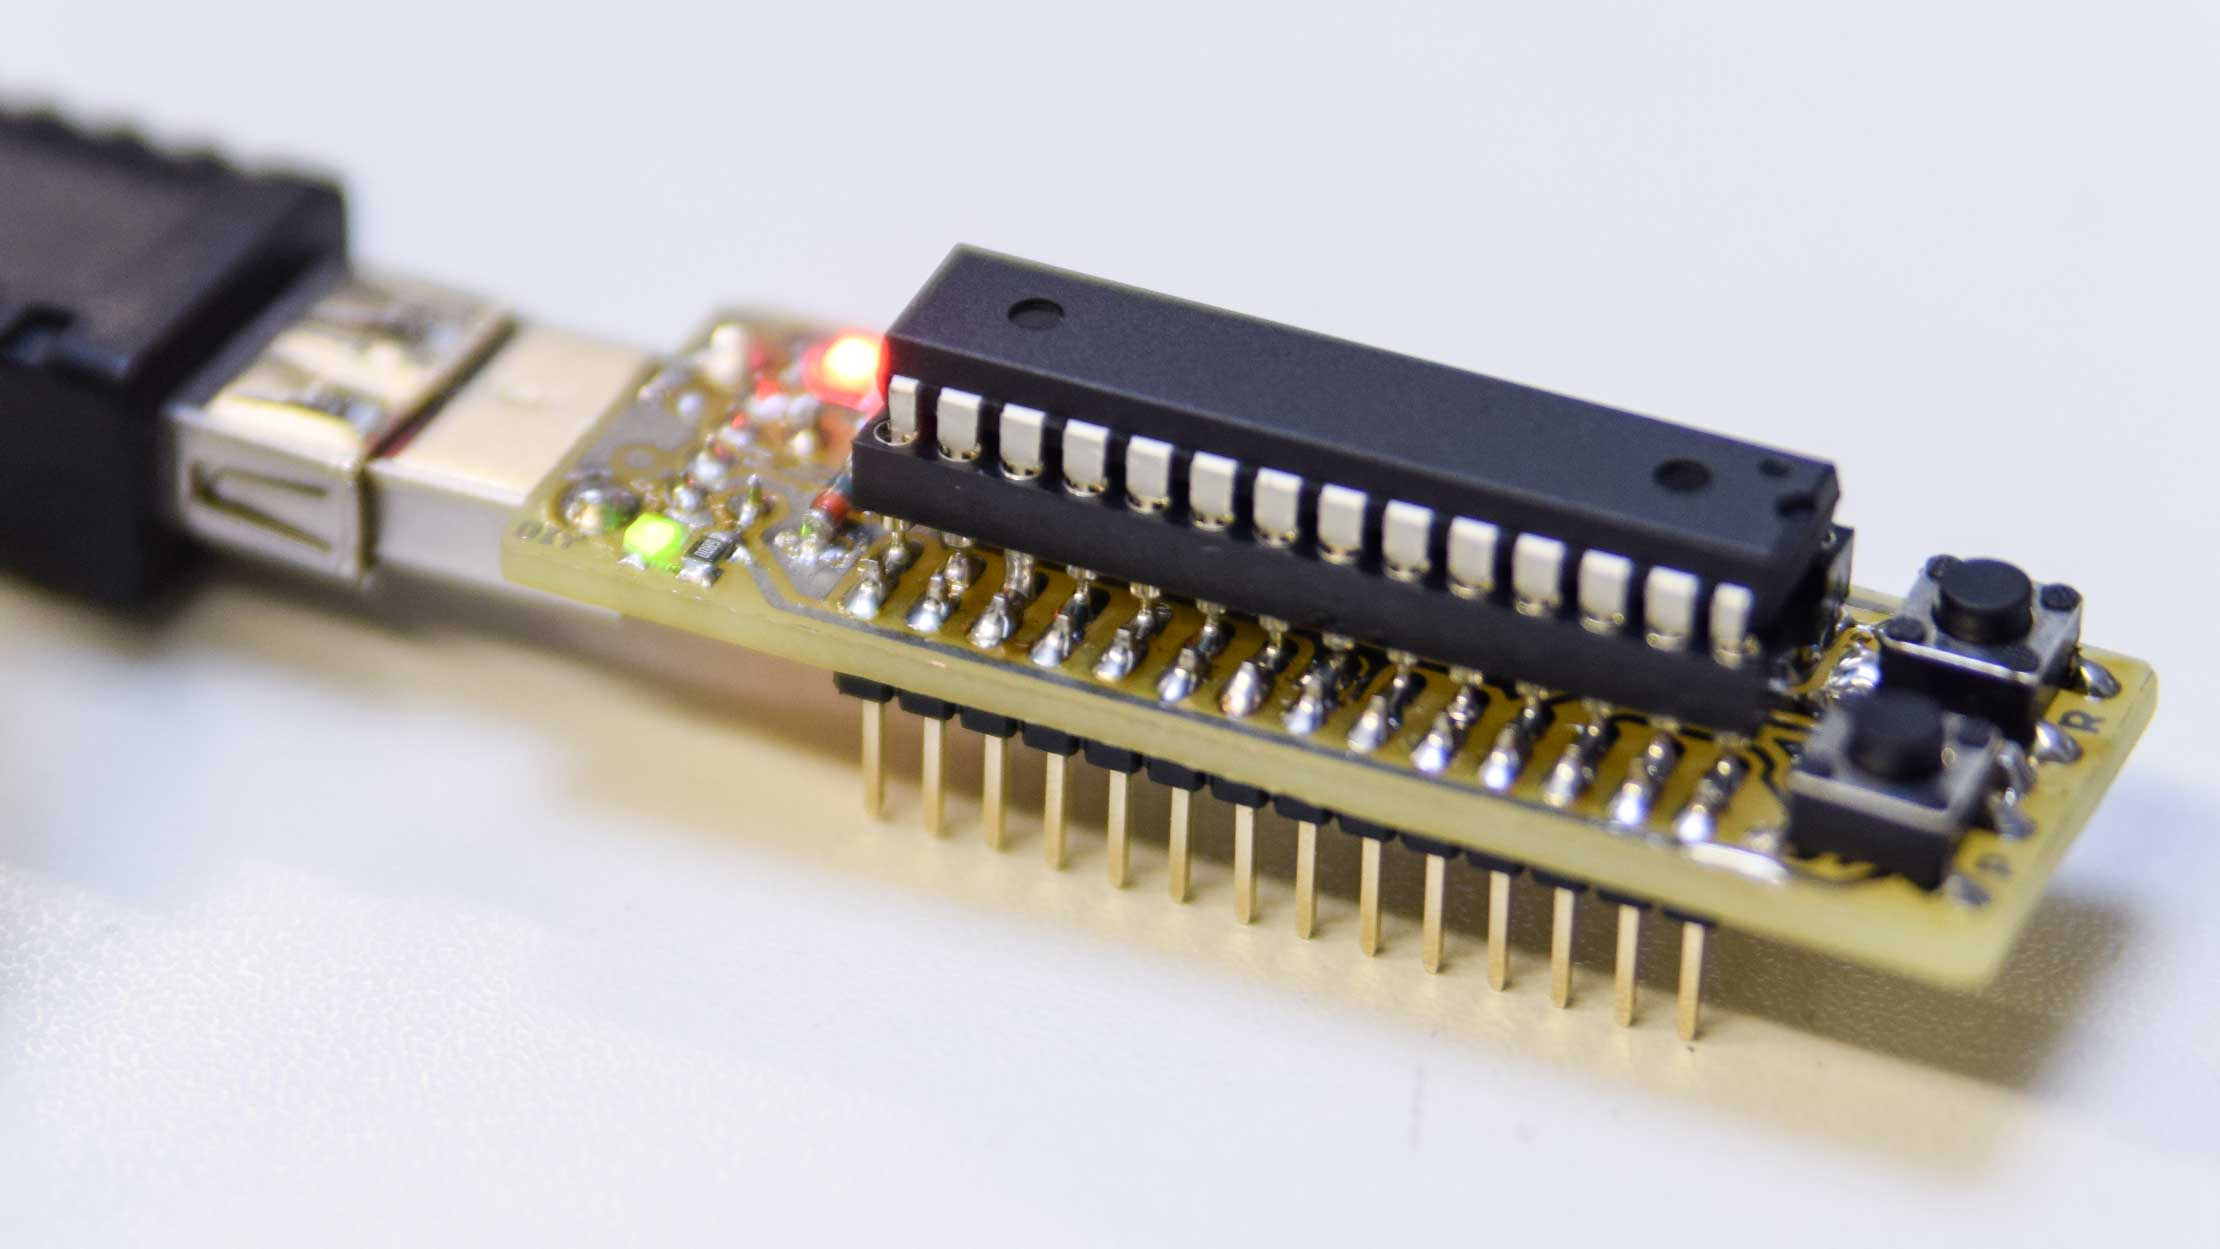
\includegraphics[width=\columnwidth]{images/diy-tinusbboard.jpg}
\section{Ätzen}
Zuerst muss das Layout auf die Platine geätzt werden.
Das Dokument spiegeln und mit möglichst hoher Tonerdichte ausgedrucken. Wenn nötig Photoplatine auf passende Größe zurecht sägen und Grate mit einer kleinen Feile entfernen. 
\paragraph*{Belichten} Die blaue Schutzfolie entfernen und auf dem gedruckten Layout im Belichter platzieren. Dabei muss die bedruckte Seite auf der beschichteten Seite der Platine aufliegen. Belichter schließen und mit empfohlene Belichtungszeit für den Belichter belichten. 
\paragraph*{Entwickeln} Mit aufgesetzter Schutzbrille die Platine, mit der beschichteten Seite nach oben, in die dafür vorgesehene Schale legen und mit etwas NaOH-Lösung begießen.
20-30 Sekunden schwenken bis keine braune Färbung mehr in die Lösung übergeht.
Platine mit einer Plastikpinzette aus der Lösung entnehmen und unter fliesendem Wasser abspülen.
\paragraph*{Ätzen} Warten bis das Ätzbad 40$^\circ$C erreicht hat. Ätzgerät ausschalten mit aufgesetzer Schutzbrille den Platinenhalter entnehmen, die Platine in den Halter einlegen. Halter in das Ätzbad stellen und Gerät wieder einschalten.
Ätzvorgang regelmäßig beobachten. Sobald alle gewünschten Stellen frei von Kupfer sind, Schutzbrille aufsetzen, Atzgerät ausschalten, Platinenhalter mit Platine entnehmen und mit Wasser abspülen.

\paragraph*{Entschichten} Platine erneut (ohne Papier ca. 2 Minuten) belichten und in die NaOH-Lösung geben. Schwenken, bis sich keine braune Farbe mehr löst.
Schale ins Waschbecken leeren und zusammen mit der Platine abspülen.
Platine im Verzinnungsbad verzinnen und erneut unter fließendem Wasser abwaschen.
\section{Bohren}
Beim Präzisionssockel kann man sich Zeit und abgebrochene Bohrer sparen, indem man nur die vier Ecken bohrt
\img{bohren.pdf}{Durchmesser der zu Bohrenden Löcher}
\section{Bestücken}
\subsection{SMT}
Die SMD Komponenten werden zuerst bestückt.
Dabei erhitzt man erst eines der Pads mit dem Lötkolben und bringt etwas Lötzinn auf. Dann wird das Bauteil mit einer Pinzette in die richtige Position gebracht. Das verzinnte Pad wird erneut erhitzt. Dann wird der andere Kontakt des Bauteils verlötet.
\paragraph*{Z-Dioden} Die Z-Dioden müssen richtig orientiert verlötet werden. Der blaue Ring markiert die Kathode der Diode. 

\img{z-dioden.pdf}{Orientierung und Position der Z-Dioden (blau)}

\paragraph*{Widerstände} Die Bauteilwerte sind auf den Widerständen aufgedruckt.
Dabei sind bei einer dreistelligen Aufschrift die ersten beiden Ziffern mit der Zehnerpotenz der dritten Ziffer zu multiplizieren. Beispiel $103 = 10 \cdot 10^3 = 10\,\mathrm{k}\Omega$\\
Bei vierstelliger Aufschrift werden die ersten drei Ziffern mit der Zehnerpotenz der letzten Ziffer multipliziert. Beispiel $6800 = 680 * 10^0 = 680\,\Omega$\\
Wird keine Zehnerpotenz angegeben wird der Buchstabe R an der Stelle des Kommas eingefügt. Beispiel $68\mathrm{R}0 = 68,0\,\Omega$
\img{widerstaende.pdf}{Position und Werte der Widerstände}

\paragraph*{Kondensatoren}
Die Kondensatoren lassen sich duch ihre Verpackung unterscheiden. Der einzige in Kunststoffhülle hat die Kapazität $1\,\mu \mathrm{F}$. Der zweier Abschnitt hat den Wert $18\,\mathrm{pF}$ und der übrige den Wert $100\, \mathrm{nF}$
\img{kondensatoren.pdf}{Position und Werte der Kondensatoren}
\paragraph*{LEDs}
Auf dem tinyUSBboard kommen eine grüne und zwei rote LEDs zum Einsatz.
\img{led-farbe.pdf}{Farben der LEDs}
\newpage
Die Kathode einer LED ist rückseitig, wie auf dem Schaltplan, mit einem Quadrat markiert.
\img{led-orientierung.pdf}{Markierung der Kathode}

\subsection{THT}
Nachdem alle SMD Komponenten verlötet sind werden die beiden Taster auf der Kupferseite verbaut.
Danach Oszillator, PTC-Widerstand und USB-Buchse; diese drei Komponenten werden von der Rückseite der Platine bestückt und auf der Kupferseite verlötet.
\img{tht.pdf}{Position THT Komponenten}

Erst wenn alle andere Komponenten mit Ausnahme der Stiftleisten verlötet sind wird der Sockel eingesetzt. Wenn nur die Löcher in den 4 Ecken gebohrt wurden müssen vor dem Löten die übrigen Pins gleichmäßig gekürzt werden.
Nachdem der Sockel verbaut ist werden zuletzt die Stiftleisten von der Unterseite bestückt und auf der Kupferseite verlötet.




